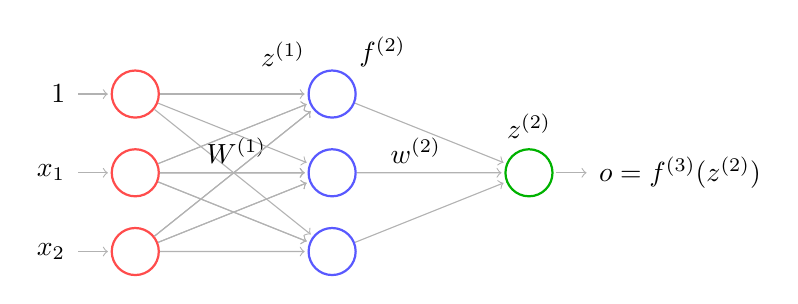
\begin{tikzpicture}[shorten >=1pt,->,draw=black!30, node distance=2.5cm]
    \tikzstyle{every pin edge}=[<-,shorten <=1pt]
    \tikzstyle{neuron}=[circle,minimum size=17pt,inner sep=0pt, line width=0.8]
    \tikzstyle{input neuron}=[neuron, draw=red!70];
    \tikzstyle{output neuron}=[neuron, draw=green!70!black];
    \tikzstyle{hidden neuron}=[neuron, draw=blue!65];
    \tikzstyle{annot} = [text width=4em, text centered]


    % Draw the input layer nodes
    \node[input neuron, pin=left: $1$] (I-0) at (0,0cm) {};
    \foreach \name / \y in {1,...,2}
      \node[input neuron, pin=left: $x_\y$] (I-\name) at (0,-\y cm) {};

    % Draw the hidden layer nodes
    \node[hidden neuron, label=above left:$z^{(1)}$, label=above right:$f^{(2)}$] (H-1) at (2.5cm,0 cm) {};
    \foreach \name / \y in {2,...,3}
      \path[yshift=1cm]
          node[hidden neuron] (H-\name) at (2.5cm,-\y cm) {};


    % Draw the output layer node
      \node[output neuron, pin={[pin edge={->,shorten <=1pt}]right: $o = f^{(3)}(z^{(2)})$},
label={above:$z^{(2)}$}] (O-1) at (5cm,-1cm) {};'

    \foreach \dest in {1,...,3}
        \path (I-0) edge (H-\dest);
    \path (I-1) edge node[above right,pos=.25]{$W^{(1)}$} (H-2);


    \path (I-1) edge (H-1);
    \path (I-1) edge (H-2);
    %\path (I-1) edge node[pos=.2]{$W^{(1)}_2$} (H-2);
    \path (I-1) edge (H-3);

    \foreach \dest in {1,...,2}
        \path (I-2) edge (H-\dest);

    \foreach \source in {1,...,2}
        \foreach \dest in {1,...,3}
            \path (I-\source) edge (H-\dest);

      \path (H-1) edge (O-1);
      \path (H-2) edge node[above,pos=.4]{$w^{(2)}$} (O-1);
      \path (H-3) edge (O-1);
\end{tikzpicture}
